\section{Latar Belakang Masalah}
\label{sec:latar_belakang}

% penggunaan natural language untuk HCI

%Bahasa alami, yang dalam \cite{depdiknas2011} juga disebut sebagai bahasa manusia, merupakan bahasa yang digunakan dalam komunikasi antar manusia baik dalam wujud tulisan, ucapan, mau pun isyarat. Seiring perkembangan teknologi komputasi, teknologi bahasa manusia (\textit{human language technology}), yang juga dikenal sebagai pemrosesan bahasa alami (\textit{natural language processing}), berusaha memanfaatkan bahasa alami untuk komunikasi yang terjadi dalam interaksi antara manusia dan komputer. Perkembangan teknologi bahasa manusia didorong oleh keinginan manusia untuk memperoleh antarmuka pengguna yang intuitif dan mudah digunakan, yang salah satunya dilakukan dengan cara menggunakan bahasa manusia saat pengguna berinteraksi dengan komputer \cite{zadrozny2000, mctear2002}.

% conversational agent (ELIZA, ALICE)

Istilah \textit{dialog system}, \textit{chatterbot}, atau \textit{conversational agent} (CA) digunakan untuk menyebut sistem komputer yang mampu bercakap-cakap dengan manusia menggunakan bahasa alami \cite{shawar2007}. Sistem ini dikenal sejak Alan Turing mendeskripsikan metode pengujian kecerdasaan buatan (kemudian dikenal sebagai \textit{Turing Test}) yang dilakukan dengan cara melakukan percakapan antara manusia dan komputer menggunakan bahasa alami \cite{turing1950}. Meskipun demikian, \textit{dialog system} sendiri baru terwujud pada pertengahan dekade 1960, ketika Joseph Weizenbaum mengembangkan ELIZA. Program yang ditujukan untuk mempelajari komunikasi antara manusia dan komputer menggunakan bahasa alami ini menganalisis dan melakukan dekomposisi teks masukan berdasarkan kata kunci yang ditemukan di dalamnya. Program kemudian menyusun tanggapan menggunakan aturan-aturan yang sesuai dengan kata kunci dan proses dekomposisi yang sebelumnya dilakukan \cite{weizenbaum1966, jurafsky2009}. Sejak kemunculan ELIZA, beberapa \textit{chatterbot} dengan pendekatan-pendekatan yang berbeda bermunculan, antara lain: PARRY, SHRDLU, MegaHAL, CONVERSE, Elizabeth, Hexbot, dan ALICE \cite{shawar2007, stephens-}. Salah satu \textit{chatterbot} yang kemudian cukup berpengaruh pada perkembangan aplikasi \textit{chatterbot} dalam satu dekade terakhir adalah \textit{Artificial Linguistic Internet Computer Entity} (ALICE). \textit{Chatterbot} yang meraih Loebner Prize, sebuah penghargaan yang diberikan kepada \textit{chatterbot} yang dinilai menyerupai manusia oleh para juri pada kontes tahunan Turing Test, pada tahun 2000, 2001, dan 2004 ini menggunakan metode pencocokan pola seperti halnya ELIZA \cite{wallace2009, loebner2011}. Selain mengembangkan sebuah \textit{chatterbot}, Richard Wallace, pengembang ALICE, juga mengembangkan \textit{Artificial Intelligence Markup Language} (AIML). Skema \textit{Extensible Markup Language} (XML) ini mempermudah pengembangan \textit{chatterbot}, terutama dalam hal membangun basis pengetahuannya. Hal ini memicu semakin banyaknya aplikasi \textit{chatterbot}, terutama yang berbasis internet, untuk berbagai keperluan, dengan berbagai basis pengetahuan, dan dalam berbagai bahasa \cite{wallace2003, gasperis2010, alice2011}.

% spoken dialog system

Perkembangan teknologi ucapan (\textit{speech technology}) memungkinkan digunakannya suara ucapan manusia sebagai masukan \textit{dialog system} dengan memanfaatkan teknologi pengenalan ucapan. Sistem yang dikenal dengan nama \textit{spoken dialog system} ini kemudian memberi tanggapan dalam suara ucapan yang dimungkinkan oleh teknologi sintesis ucapan. Singkatnya, komunikasi dengan bahasa alami antara manusia dan komputer pada \textit{spoken dialog system} berbasis ucapan, tidak lagi berbasis teks seperti pada \textit{dialog system} terdahulu. Selain perkembangan antarmuka tersebut, perkembangan juga terjadi pada metode penyusunan tanggapan. Pada \textit{spoken dialog system}, dikenal adanya \textit{dialog manager}. \textit{Dialog manager} berperan seperti bagian pencocokan pola pada ELIZA. Akan tetapi, berbeda dengan metode pencocokan pola pada ELIZA yang hanya mempertimbangkan masukan yang akan ditanggapi, \textit{dialog manager} pada \textit{spoken dialog system} mempertimbangkan konteks percakapan, yang disimpulkan dari percakapan yang terjadi sebelumnya, dalam menyusun tanggapan \cite{mctear2002, jurafsky2009, cole1997}.

% embodied conversational agent (ECA) dan implementation of ECA (museum, tour guide, etc.)

\textit{Conversational agent}, yang sebelumnya hanya mampu menerima masukan dan memberi keluaran dalam bentuk teks atau suara saja, kemudian berevolusi menjadi \textit{conversational agent} yang memiliki wujud, misalnya berupa karakter manusia dalam bentuk 3-dimensi (3D), yang dikenal sebagai \textit{embodied conversational agent} (ECA) atau \textit{embodied conversational interface agent}. Wujud yang dimiliki oleh agen memungkinkan lebih banyak cara yang dapat digunakan dalam komunikasi antara manusia dan komputer, misalnya arah tatapan mata, gerakan badan, dan mimik muka. Dengan kata lain, agen memiliki kemampuan untuk melakukan komunikasi non-verbal dengan pengguna, seperti yang dilakukan dalam komunikasi tatap muka antar manusia, sehingga berpotensi menciptakan komunikasi yang lebih alami dan pengalaman interaksi yang lebih kaya bagi penggunanya \cite{beun2003, cassell1999, cassell2000, cassell2000a, rehm2005, rickel2002, foster2007}. Beberapa contoh implementasi ECA, antara lain: agen serba guna Greta \cite{niewiadomski2009}, agen properti REA \cite{cassell1999}, tutor pembelajaran bahasa Baldi \cite{massaro2006}, dan pemandu museum Ada dan Grace \cite{swartout2010}. Ada dan Grace, yang namanya diambil dari Ada Lovelace dan Grace Hopper (dua tokoh wanita di sejarah perkembangan komputer), merupakan agen pemandu museum virtual yang ada di Museum of Science, Boston, tepatnya di bagian "InterFaces" yang memamerkan benda-benda bersejarah di bidang komputer, robotika, dan teknologi komunikasi. Ada dan Grace dapat menjawab pertanyaan pengunjung, menjelaskan dan menyarankan suatu benda museum, serta menjelaskan bagaimana sistem dialog mereka bekerja (\autoref{fig:ada_grace}). Pengetahuan dan karakter kedua agen didesain berbeda untuk memungkinkan terjadinya dialog yang lebih hidup dan memberikan pengalaman yang lebih kaya bagi pengunjung saat menjelajah museum \cite{themuseumofscienceboston-, uscinstituteforcreativetechnologies-}.

\begin{figure}[ht!]
\vskip 1em
\centering
 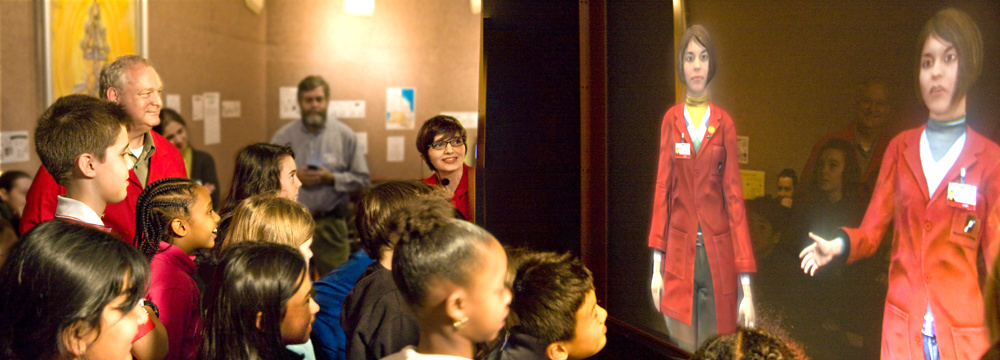
\includegraphics[width=0.9\textwidth,keepaspectratio=true]{images/ada_grace.jpg}
 \caption[Interaksi pemandu museum virtual Ada dan Grace dengan pengunjung di Museum of Science, Boston]{Interaksi pemandu museum virtual Ada dan Grace dengan pengunjung di Museum of Science, Boston \cite{armedwithscience-}.}
 \label{fig:ada_grace}
\vskip .5em
\end{figure}

Secara umum, implementasi ECA belum terlihat di Indonesia. Padahal, ECA dapat dimanfaatkan di berbagai bidang, misalnya di bidang pendidikan dan bidang pariwisata. ECA dapat dimanfaatkan sebagai tutor dalam proses pembelajaran. ECA juga dapat dimanfaatkan untuk membangun kios informasi pariwisata yang kemudian dapat ditempatkan di lokasi-lokasi yang mudah dijangkau oleh wisatawan, seperti di bandara, stasiun, terminal, hotel, atau bahkan di objek pariwisatanya sendiri. Implementasi ECA sebagai pemandu museum seperti Ada dan Grace dapat juga dilakukan di Indonesia untuk menarik lebih banyak orang untuk mengunjungi museum mengingat jumlah rata-rata pengunjung museum-museum di Indonesia pada kurun waktu 2006-2008 hanya mencapai 4,3 juta atau hanya 1,8 persen dari 237 juta lebih penduduk Indonesia (data tahun 2010) \cite{dppobappenas2009, bps2010}.

% RESTU's an Engine for Synthetic Thespian Units

Oleh karena itu, tim PUSPA dan SAMsON dari Program Magister Teknik Elektro, Sekolah Teknik Elektro dan Informatika (STEI), Institut Teknologi Bandung (ITB) bekerjasama dalam mengembangkan \textit{RESTU's an Engine for Synthetic Thespian Units} (RESTU), yang merupakan \textit{engine} untuk membangun ECA. Sebagai sebuah \textit{engine}, RESTU terdiri dari bagian interaksi dan bagian kognisi. Secara umum, bagian interaksi memanfaatkan monitor untuk menampilkan wujud agen, mikrofon sebagai telinga, kamera sebagai mata, dan speaker sebagai mulut. Sedangkan, bagian kognisi dapat dipilih untuk memanfaatkan AIML atau menggunakan \textit{artificial general intelligence} (AGI). Tim PUSPA sendiri memiliki tujuan membangun \textit{PUSPA’s an Understanding Synthespian that Provides Assistance} (PUSPA), yaitu sebuah ECA yang berperan sebagai asisten pribadi. Sedangkan, tim SAMsON memiliki tujuan membangun \textit{Smart Assistant for Museum's Objects Navigation} (SAMsON), yaitu sebuah ECA yang berperan sebagai pemandu museum \cite{nugraha2010}.

\begin{figure}[ht!]
\vskip 1em
\centering
 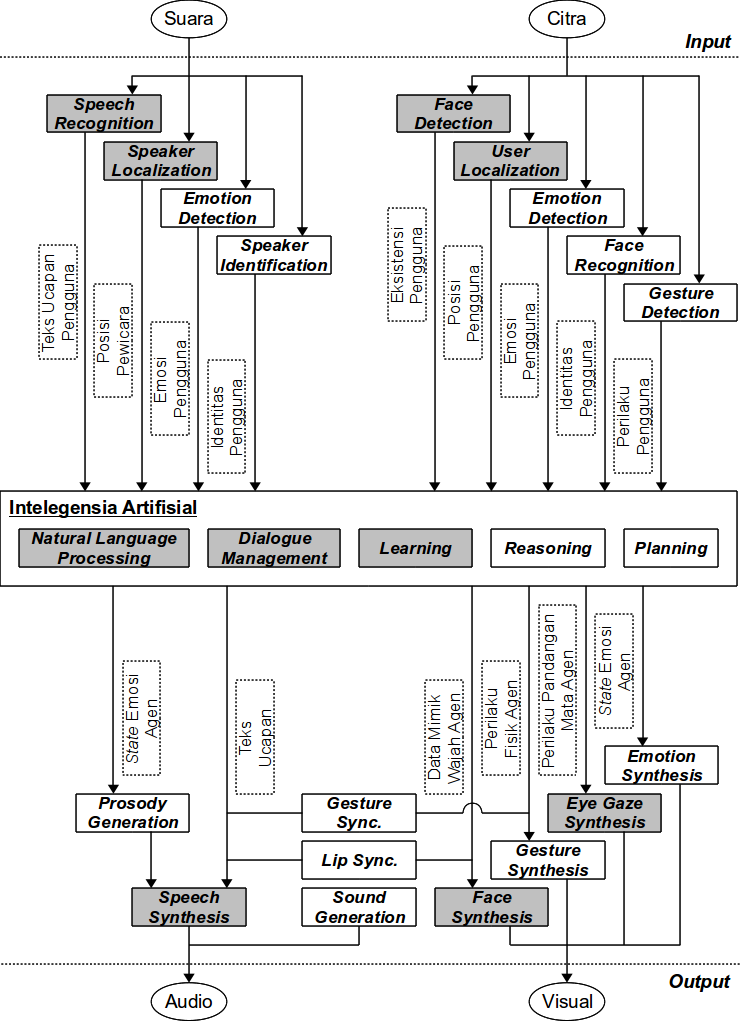
\includegraphics[width=\textwidth,keepaspectratio=true]{images/diagram_blok_eca.png}
 \caption[Diagram blok teknologi penyusun RESTU]{Diagram blok teknologi penyusun RESTU.}
 \label{fig:diagram_blok_eca}
\vskip .5em
\end{figure}

\autoref{fig:diagram_blok_eca} menunjukkan berbagai teknologi terkait ECA yang dapat diimplementasikan pada RESTU. Pada saat ini, teknologi yang diimplementasikan masih terbatas pada teknologi-teknologi yang dalam \autoref{fig:diagram_blok_eca} diberi \textit{background} berwarna abu-abu. Di luar teknologi-teknologi yang sudah tercantum, masih banyak teknologi yang berpotensi meningkatkan kemampuan interaksi ECA. Sebagai contoh, pada pengolahan masukan berupa suara (ucapan), terdapat teknologi \textit{speaker segmentation} dan \textit{speaker tracking}. Implementasi kedua teknologi ini pada RESTU akan memberi kemampuan pada ECA yang dihasilkan untuk mengelola komunikasi dengan pengguna lebih dari satu (\textit{multi-speaker environment}) \cite{martin2001}.

Seperti yang dapat dilihat pada \autoref{fig:diagram_blok_eca}, pada dasarnya komunikasi antara ECA dengan penggunanya hanya memanfaatkan media suara (audio) dan gambar (visual). Meskipun demikian, dari media audiovisual ini, berbagai komunikasi non-verbal dapat berlangsung, misalnya emosi pengguna dapat diketahui dari intonasi suaranya, ekspresi wajahnya, sikap tubuhnya, atau tatapan matanya. Di sisi lain, agen virtual juga dapat menunjukkan emosi yang beragam dengan memberi intonasi tertentu pada suara yang dihasilkan, ekspresi wajah tertentu, sikap tubuh serta pergerakan anggota badan tertentu, atau bahkan dengan tatapan mata tertentu \cite{morency2006, hartmann2005}.


% natural communication: face-to-face, implementation in ECA (need to know speaker location)

Dalam komunikasi tatap muka antar manusia, tatapan mata berperan penting dalam komunikasi non-verbal. Contoh yang paling sederhana adalah tatapan mata dapat memberi petunjuk kepada siapa seseorang sedang berbicara dan dapat memberi petunjuk kondisi emosi seseorang. Oleh karena ECA memiliki wujud, termasuk mata, tatapan mata sebagai salah satu metode komunikasi non-verbal ini juga dapat diimplementasikan untuk menciptakan komunikasi antara manusia dan komputer yang sama alaminya dengan komunikasi antar manusia. Implementasi tatapan mata dan pergerakan mata yang berbeda pada ECA juga telah terbukti memberikan kesan dan tingkat kepuasan yang berbeda bagi penggunanya \cite{lee2002, vanes2002}. Oleh karena itu, sebagai \textit{engine} ECA, RESTU juga harus mengakomodasi fitur ECA yang berupa tatapan dan pergerakan mata agen.

% source localization

Informasi yang dibutuhkan oleh agen dalam menentukan ke arah mana mata agen harus menatap adalah lokasi pengguna atau lawan bicara agen. Dalam RESTU, penentuan lokasi pengguna mungkin dilakukan dengan memanfaatkan informasi yang didapatkan dari: (1) sinyal suara yang ditangkap oleh mikrofon; dan/atau (2) citra yang ditangkap oleh kamera. Mempertimbangkan persyaratan \textit{modularity} dan \textit{extensibility} terkait modalitas masukan dan keluaran yang termasuk dalam persyaratan arsitektur ECA seperti yang tercantum dalam \cite{cassell1998}, penentuan lokasi pengguna dalam RESTU juga harus dapat dilakukan hanya berdasarkan sinyal suara saja atau gambar saja. Meskipun demikian, hasil penentuan lokasi kedua metode tersebut juga dapat dikombinasikan untuk memperoleh lokasi pengguna yang lebih akurat. Penentuan lokasi menggunakan citra yang ditangkap kamera cenderung menghasilkan nilai posisi yang lebih akurat. Akan tetapi, area dimana metode ini dapat digunakan lebih sempit dibandingkan area dimana metode penentuan lokasi menggunakan suara dapat digunakan. Analogi sederhananya adalah telinga manusia dapat mendengar suara yang berasal dari suatu posisi yang terletak di luar jangkauan pandangan mata, misalnya sebuah posisi yang terletak di belakang kepala.
